\chapter{TP1:Présentation et programmation de la carte Arduino}
\minitoc
\newpage
\section{Matériel}

Le projet Arduino a été conçu par une équipe de six développeurs pour offrir une plateforme de création de systèmes électroniques accessible à tous, des débutants aux professionnels.

\begin{figure}[H]
	\centering
	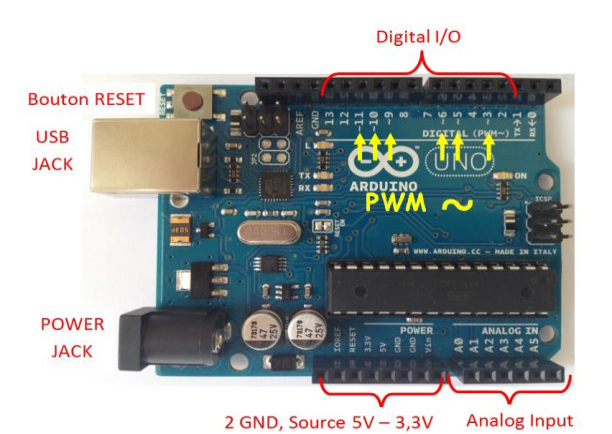
\includegraphics[width=0.7\linewidth]{Image/1.Arduino_Uno}
	\caption{Arduino Uno}
	\label{fig:arduinouno}
\end{figure}

La carte Arduino UNO est un circuit imprimé architecturé autour du microcontrôleur ATmega328. Elle est équipée d'une interface USB permettant une communication directe avec un ordinateur. 

\paragraph{Caractéristiques techniques principales :}
\begin{itemize}
	\item \textbf{Tensions :} Fonctionnement sous 5V, avec une tension d'alimentation recommandée de 7 à 12V.
	\item \textbf{Performances :} Horloge cadencée à 16~MHz et mémoire Flash de 32~Ko.
	\item \textbf{Courant :} Jusqu'à 40~mA par broche d'entrée/sortie (50~mA pour la broche 3.3V).
	\item \textbf{Brochage :}
	\begin{itemize}
		\item \emph{Entrées analogiques :} A0 à A5
		\item \emph{Entrées/Sorties numériques :} 2 à 19
		\item \emph{Sorties PWM (analogiques simulées) :} 3, 5, 6, 9, 10, 11
	\end{itemize}
\end{itemize}
\section{Le logiciel Arduino}
La programmation de la carte Arduino nécessite un logiciel pour écrire le code puis le transférer. Nous utiliserons pour cela Arduino IDE, une solution gratuite et open source.
\begin{figure}[H]
	\centering
	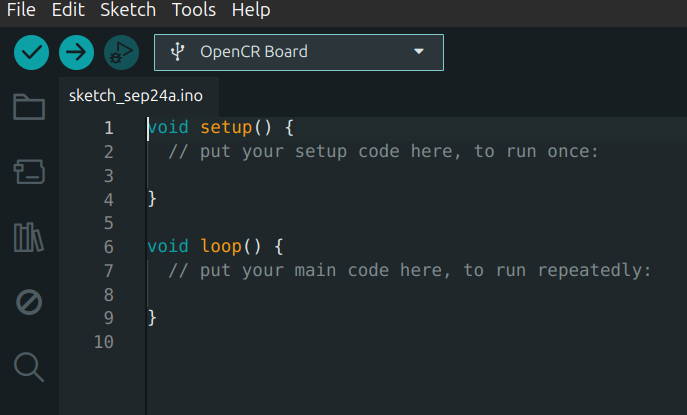
\includegraphics[width=0.7\linewidth]{Image/1.Interface_IDE}
	\caption{Interface Arduino IDE}
	\label{fig:interfaceide}
\end{figure}

\section{Manipulation}
\subsection{Manipulation 1 : Une LED qui clignote}
Le but de cette première manipulation est de nous familiariser avec la carte Arduino Uno en faisant simplement clignoter une LED.
\begin{figure}[H]
	\centering
	\begin{minipage}{0.48\textwidth}
		\centering
		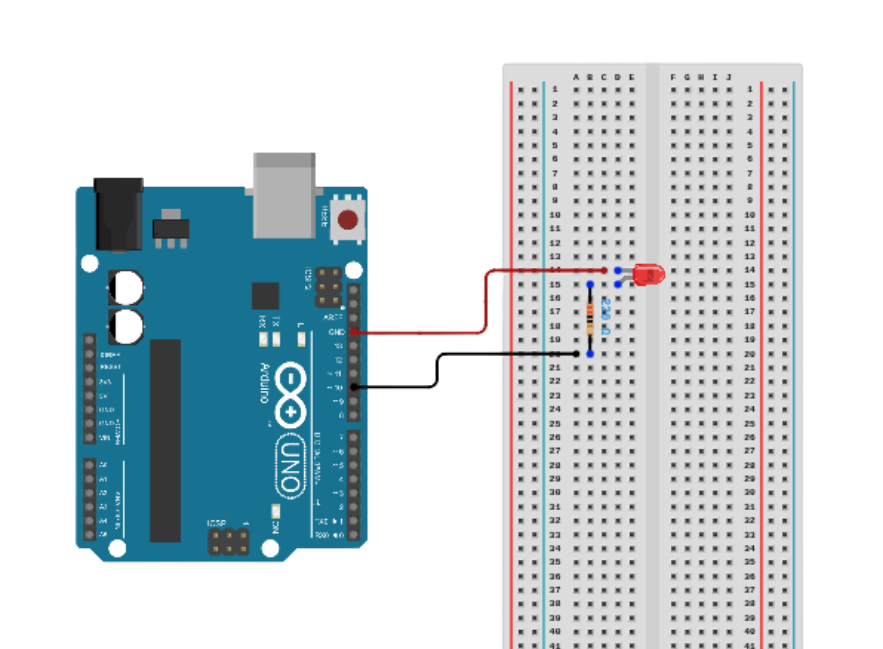
\includegraphics[width=\linewidth]{Image/1.Schéma_Manip1}
		\caption{Schéma Manipulation 1}
		\label{fig:schemamanip1}
	\end{minipage}\hfill
	\begin{minipage}{0.48\textwidth}
		\centering
		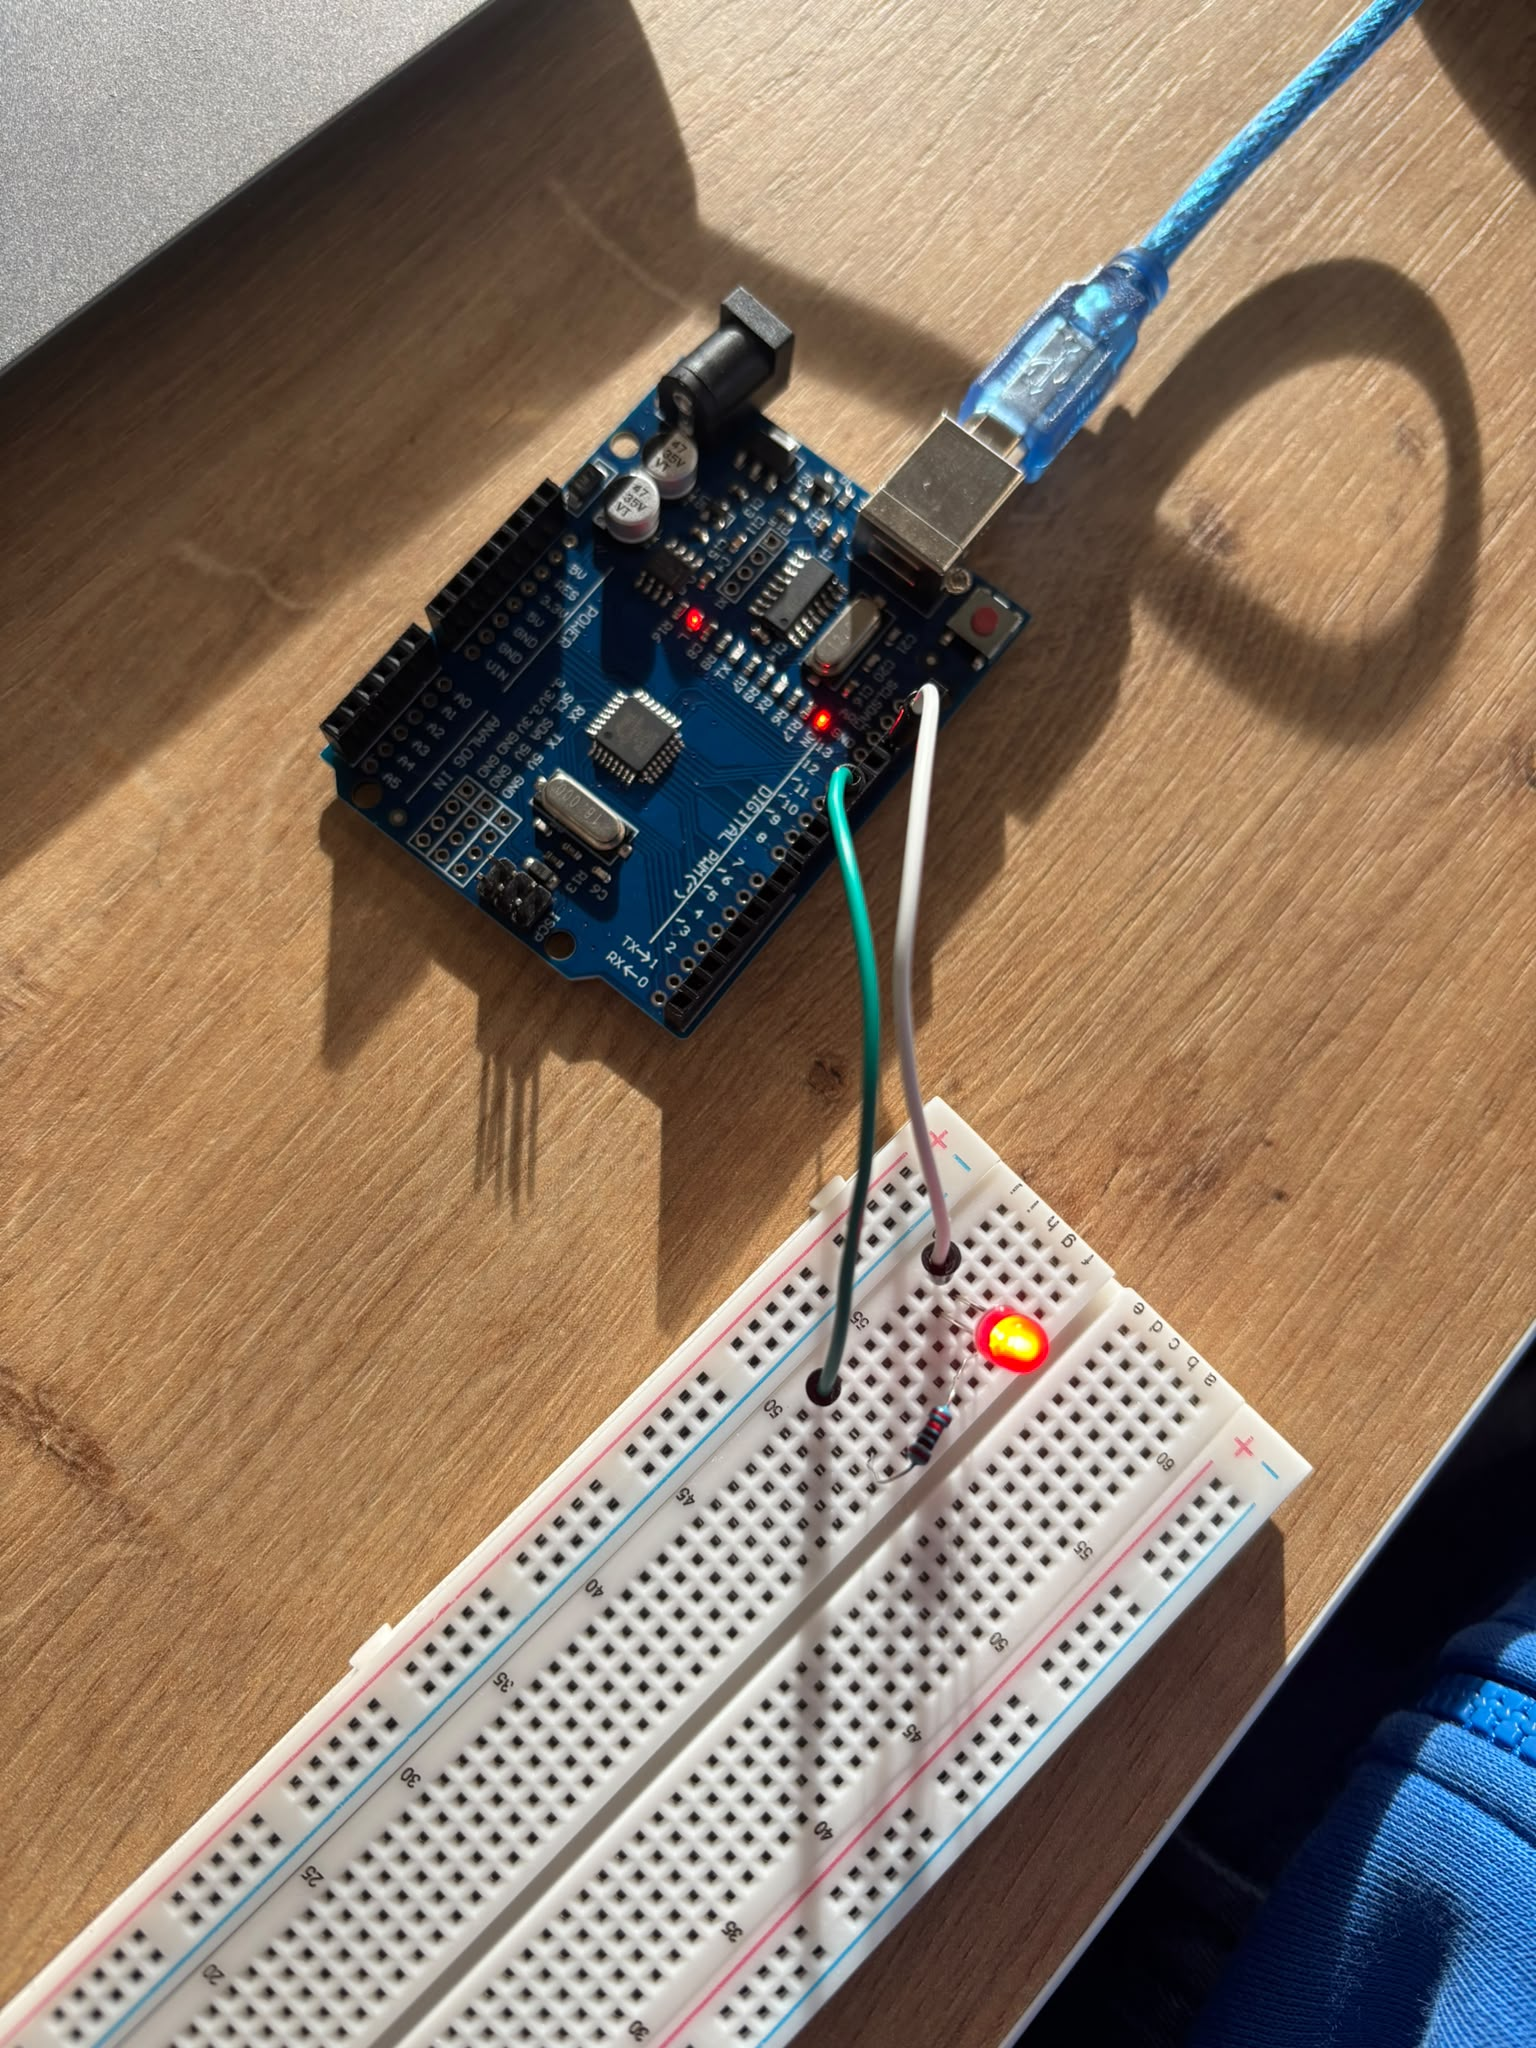
\includegraphics[width=\linewidth]{Image/1.Photo_manip1}
		\caption{Photo Manipulation 1}
		\label{fig:photomanip1}
	\end{minipage}
\end{figure}
Voici le code qui nous est donné pour tester notre LED
\begin{lstlisting}
	void setup() {		
		pinMode(10, OUTPUT); // ici nous definissons notre pin 10 comme une sortie 		
	}	
	void loop() {		
		digitalWrite(10, HIGH); // ici on allume la LED
		delay(500); // on attends 500 millisecondes
		digitalWrite(10, LOW);
		delay(500); // on attends 500 millisecondes		
	}
		
\end{lstlisting}
\textbf{Observation :} Nous remarquons bien que la LED clignote. 

\subsection{Manipulation 2 : Trois LED qui clignote}
Dans cette partie du TP, nous devons apprendre à gérer trois LED en même temps avec notre Arduino.
\begin{figure}[H]
	\centering
	% Première image à gauche (48% de la largeur de la page)
	\begin{minipage}{0.48\textwidth}
		\centering
		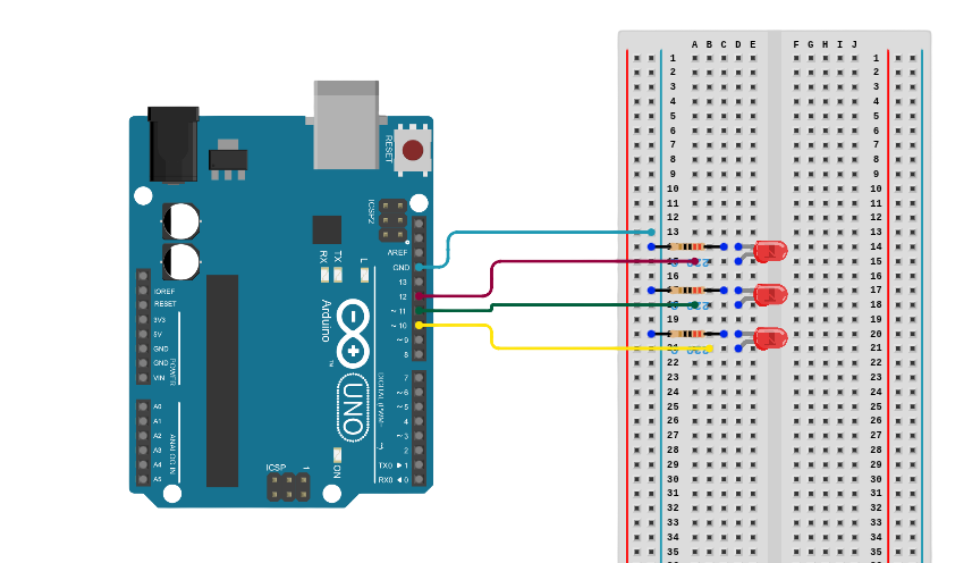
\includegraphics[width=\linewidth]{Image/1.Schéma_manip2}
		\caption{Schéma manipulation 2}
		\label{fig:schemamanip2}
	\end{minipage}\hfill
	% Seconde image à droite (48% de la largeur de la page)
	\begin{minipage}{0.48\textwidth}
		\centering
		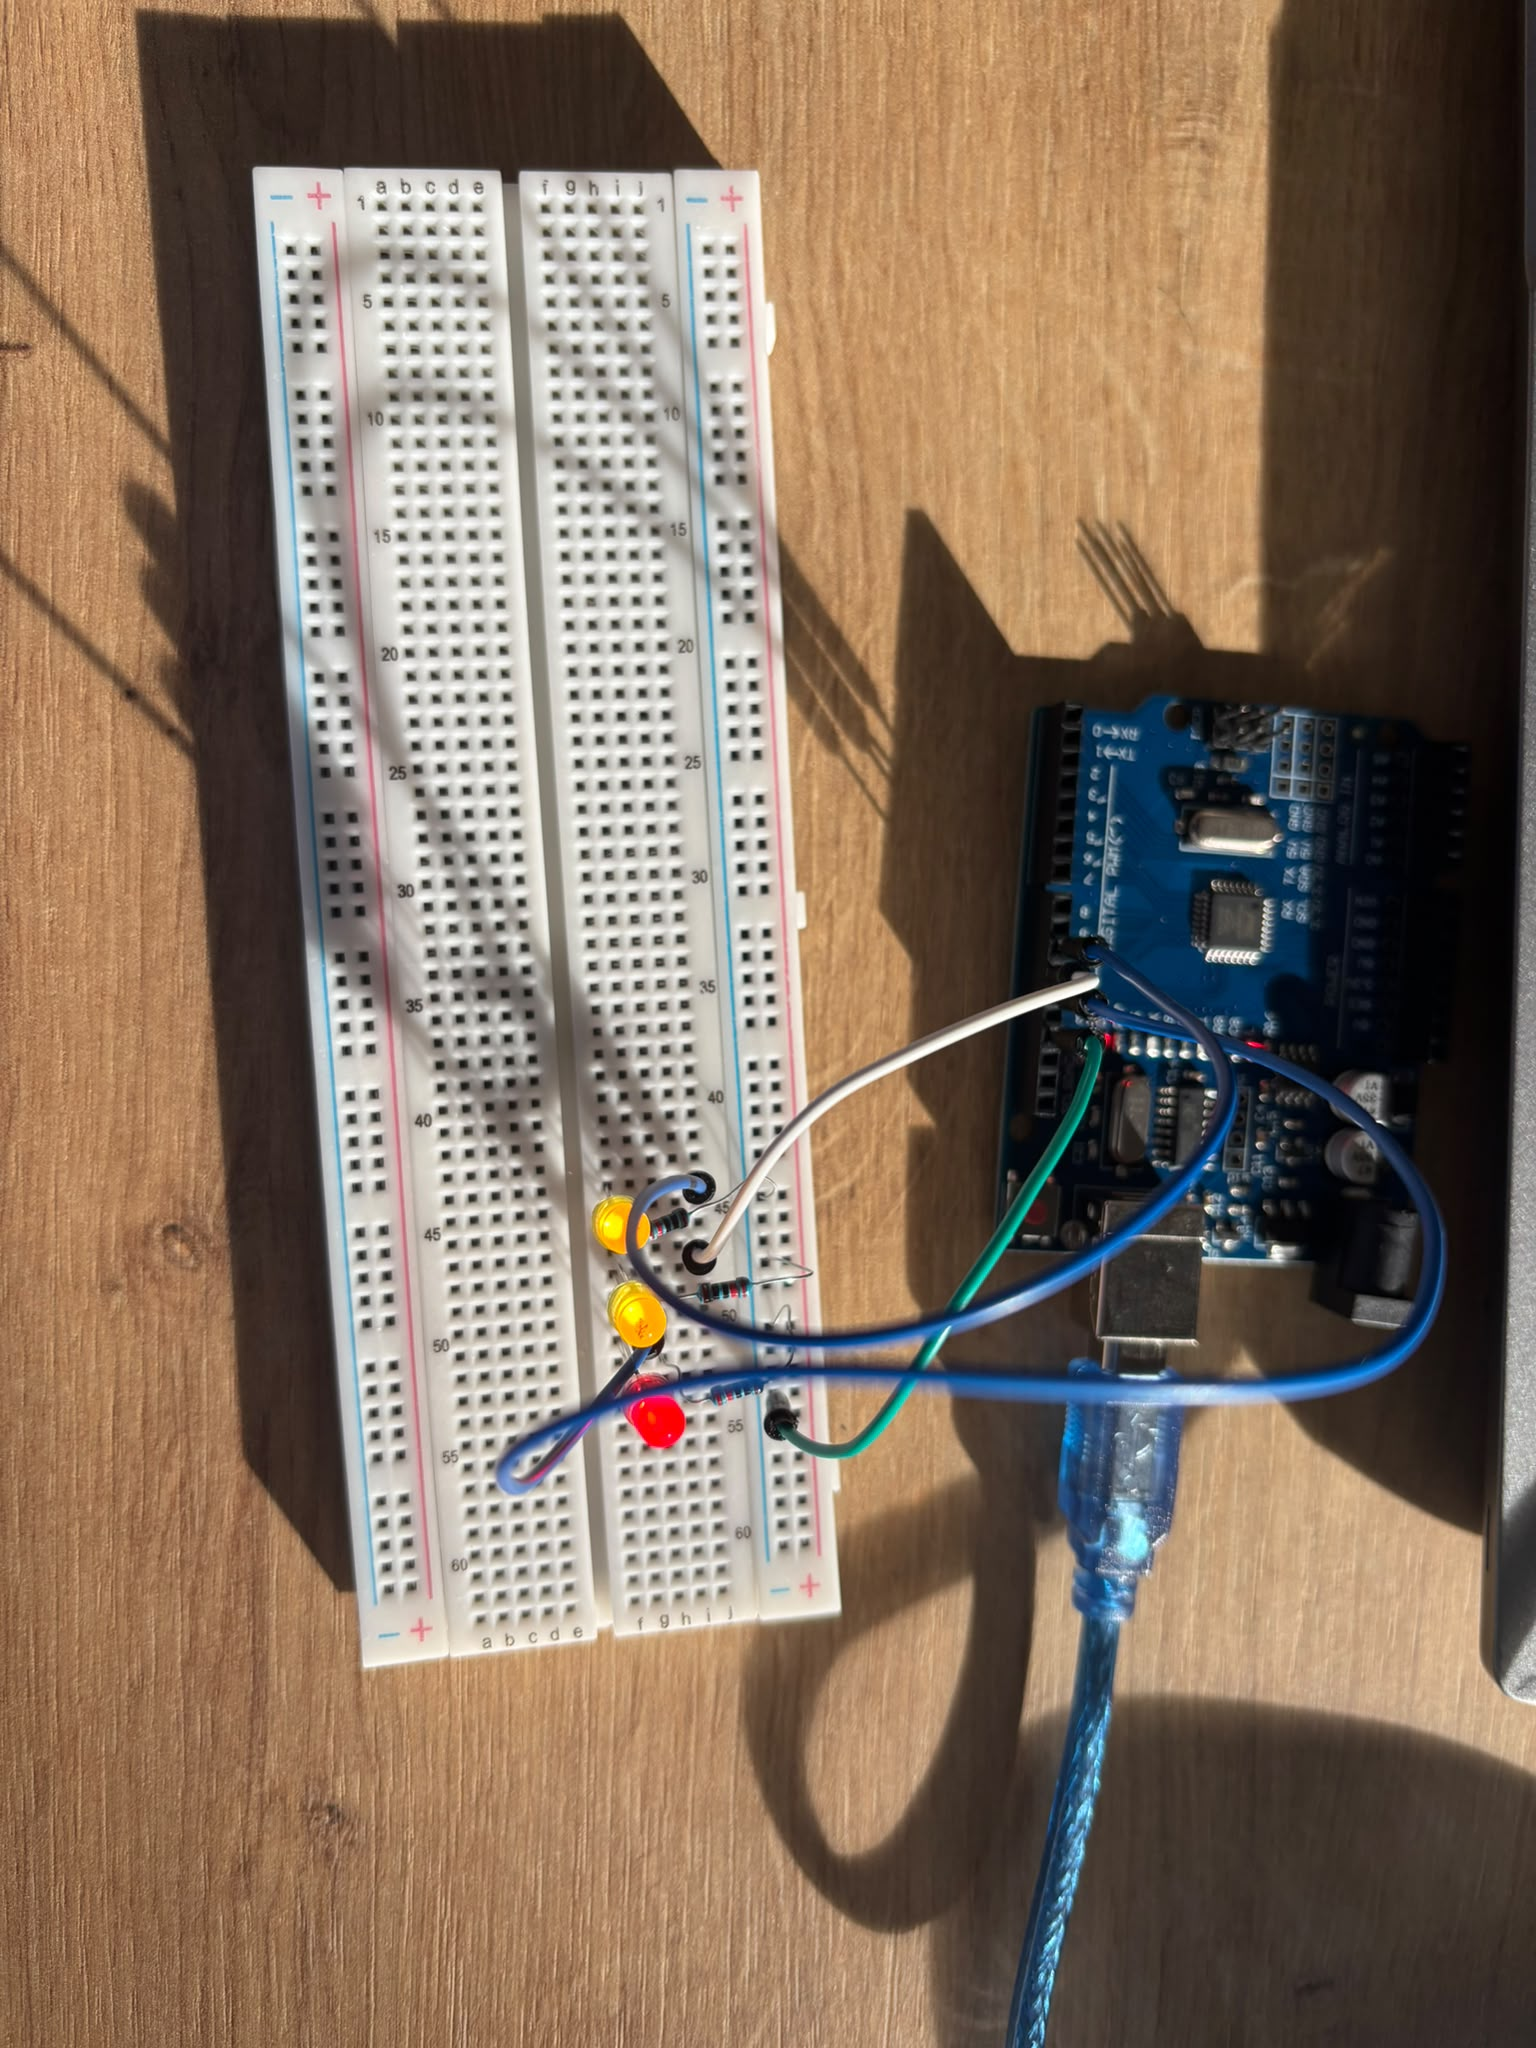
\includegraphics[width=\linewidth]{Image/1.Photo_manip2}
		\caption{Photo Manipulation 2}
		\label{fig:photomanip2}
	\end{minipage}
\end{figure}
Voici notre code pour faire code pour faire clignoter les trois LED
\begin{lstlisting}	
	void setup() {
		pinMode(10, OUTPUT); // ici nous definissons notre pin 10 comme une sortie 
		pinMode(11, OUTPUT); // ici nous definissons notre pin 11 comme une sortie 
		pinMode(12, OUTPUT); // ici nous definissons notre pin 12 comme une sortie 
	}
	void loop() {
		digitalWrite(10, HIGH); // ici on allume la LED
		digitalWrite(11, HIGH); // ici on allume la LED
		digitalWrite(12, HIGH); // ici on allume la LED
		
		delay(500); // on attends 500 millisecondes
		
		digitalWrite(10, LOW);
		digitalWrite(11, LOW);
		digitalWrite(12, LOW);
		
		delay(500); // on attends 500 millisecondes		
	}	
\end{lstlisting}
\textbf{Observation :} Nous remarquons que les trois LED s'allume simultanément.\\
Ensuite nous devons faire en sorte que les trois Led s'allume avec alternance. Voici le code pour faire cela. 
\begin{lstlisting}	
	void loop() {		
		digitalWrite(10, HIGH); // ici on allume la LED
		delay(500); // on attends 500 millisecondes
		digitalWrite(10, LOW); // ici on allume la LED
		
		delay(500);
		
		digitalWrite(11, HIGH); // ici on allume la LED
		delay(500); // on attends 500 millisecondes
		digitalWrite(11, LOW); // ici on allume la LED
		
		delay(500);
		
		digitalWrite(12, HIGH); // ici on allume la LED
		delay(500); // on attends 500 millisecondes
		digitalWrite(12, LOW); // ici on allume la LED
		
		delay(500);
	}	
\end{lstlisting}
\textbf{Observations :} Nous remarquons bien une alternance dans l'allumage des LED.\\
Pour la prochaine questions nous devons réaliser un feu tricolore avec nos trois LED de couleur. Voici alors notre code pour réaliser cela.
\begin{lstlisting}		
	#define LED_rouge  12 // ici nous renommons nous leds pour mieux les distinguer
	#define LED_vert   11
	#define LED_orange 10	
	void setup() {		
		pinMode(LED_rouge, OUTPUT); 
		pinMode(LED_vert, OUTPUT); 
		pinMode(LED_orange, OUTPUT); 
	}	
	void loop() {
		
		digitalWrite(LED_orange, HIGH); 
		digitalWrite(LED_vert, LOW);
		digitalWrite(LED_rouge, LOW);
		
		delay(1000);
		
		digitalWrite(LED_orange, LOW);
		digitalWrite(LED_vert, LOW);
		digitalWrite(LED_rouge, HIGH);
		
		delay(4000);
		
		digitalWrite(LED_orange, LOW); 
		digitalWrite(LED_vert, HIGH);
		digitalWrite(LED_rouge, LOW);
		
		delay(4000);		
	}		
\end{lstlisting}
\textbf{Observations :} Nous remarquons bien le fait que les LED s'allume a l'image d'un feux tricolore.\\
L'exercice suivant consiste à répéter 15 fois le clignotement d'une seule LED. Pour éviter d'alourdir le programme, nous allons conserver notre structure actuelle et introduire une boucle for. 
\begin{lstlisting}			
	void setup() {
		Serial.begin(9600);
		
		pinMode(10, OUTPUT); 
				
		for(int i=0 ; i <15 ; i++){ // cette boucle for nous permet d'executer le code 15 fois 
			Serial.println(i);
			digitalWrite(10,HIGH);
			delay(500);
			digitalWrite(10,LOW);
			delay(500);			
		}
	}	
	void loop() {		
		// ici on ne mets rien car on souhaite que le code sexecute que 15 fois		
	}
\end{lstlisting}
\textbf{Observations :} Nous vérifions bien que la LED s’allume et s’éteint 15 fois.\\
Nous avons désormais un code a tester.
\begin{lstlisting}				
	int ledPin = 10; //On renomme la broche 10 en "ledPin"
	int timer = 100; //On definit une duree de 0,1 seconde pour la variable timer
	
	void setup() { pinMode(ledPin, OUTPUT); }
	
	void loop() {		
		// LED a 0%.
		analogWrite(ledPin, 0);
		delay(timer);
		// LED a 19.6%.
		analogWrite(ledPin, 50);
		delay(timer);
		// LED a 39.2%.
		analogWrite(ledPin, 100);
		delay(timer);
		// LED a 58.8%.
		analogWrite(ledPin, 150);
		delay(timer);
		// LED a 78.4%.
		analogWrite(ledPin, 200);
		delay(timer);
		// LED a 100%.
		analogWrite(ledPin, 255);
		delay(timer); }
\end{lstlisting}
\textbf{Observations :} La LED augmente en luminosité jusqu’à s'éteindre.\\
Maintenant que nous avons compris ce précedent code nous devons jouer avec la luminosité des Trois différente LED.
\begin{lstlisting}					
	int ledPin = 10; //On renomme la broche 10 en "ledPin"
	int timer = 100; //On definit une duree de 0,1 seconde pour la variable timer
	
	void setup() {
		pinMode(ledPin, OUTPUT);
	}
	
	void loop() {
		analogWrite(10, (255*10)/100); // ici on definit la luminosite de la led_10 a 10% de 255
		analogWrite(11, (255*40)/100); // ici on definit la luminosite de la led_11 a 40% de 255
		analogWrite(12, (255*80)/100); // ici on definit la luminosite de la led_12 a 80% de 255
		
		delay(timer);
		
		analogWrite(10, (255*0)/100); // ici on definit la luminosite de la led_10 a 0% de 255
		analogWrite(11, (255*0)/100); // ici on definit la luminosite de la led_11 a 0% de 255
		analogWrite(12, (255*0)/100); // ici on definit la luminosite de la led_12 a 0% de 255		
		
		delay(timer);		
	}
\end{lstlisting}
\textbf{Observations :}Les trois LED clignote mais avec une intensité lumineuse différente.\\
Pour finir avec ce TP nous allons réaliser un chenillard avec nos trois LED. 
\begin{lstlisting}						
	int timer = 500; //On definit une duree de 0,5 seconde pour la variable timer	
	void setup() {
		pinMode(10, OUTPUT);
		pinMode(11, OUTPUT);
		pinMode(12, OUTPUT);
	}	
	void loop() {		
		for (int i = 10 ; i < 13 ; i++) {			
			digitalWrite(i, HIGH);
			delay(timer);
			digitalWrite(i, LOW);			
		}		
	}
\end{lstlisting} 
\textbf{Observations :} Nous observons bien l'allumage des LED de façons successive.